\documentclass[tikz]{standalone}
\usepackage[utf8]{inputenc}
\usetikzlibrary{calc}

\definecolor{mycolor}{RGB}{12,18,33}

\begin{document}
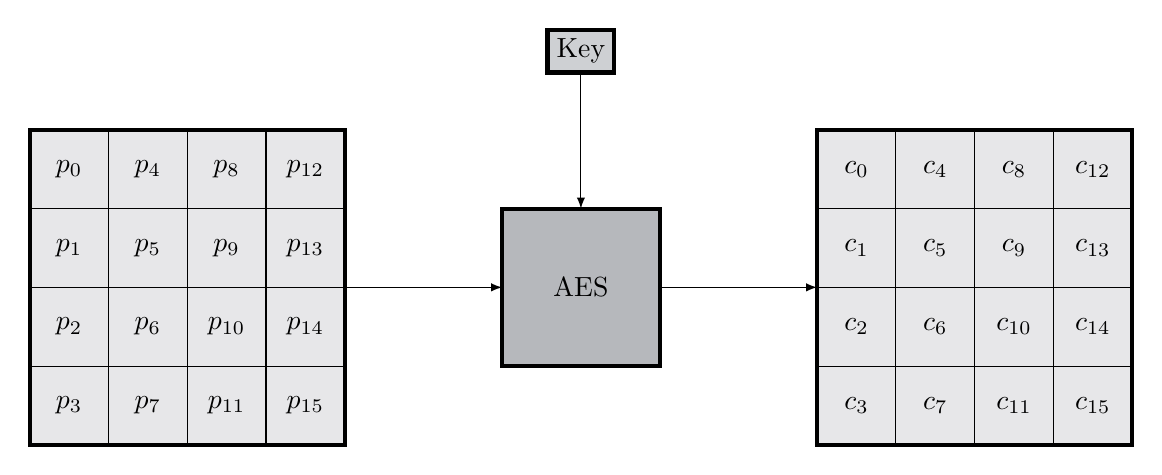
\begin{tikzpicture}
% plaintext
\foreach\x in {0, 1, ..., 3}
\foreach\y in {0, 1, ..., 3}
\draw[fill=mycolor!10] (\x,\y) rectangle ($(\x,\y) + (1,1)$);

\draw[line width=1.5pt] (0,0) rectangle (4,4);
\node at (0.5, 0.5) {$p_3$};
\node at (0.5, 1.5) {$p_2$};
\node at (0.5, 2.5) {$p_1$};
\node at (0.5, 3.5) {$p_0$};
\node at (1.5, 0.5) {$p_7$};
\node at (1.5, 1.5) {$p_6$};
\node at (1.5, 2.5) {$p_5$};
\node at (1.5, 3.5) {$p_4$};
\node at (2.5, 0.5) {$p_{11}$};
\node at (2.5, 1.5) {$p_{10}$};
\node at (2.5, 2.5) {$p_9$};
\node at (2.5, 3.5) {$p_8$};
\node at (3.5, 0.5) {$p_{15}$};
\node at (3.5, 1.5) {$p_{14}$};
\node at (3.5, 2.5) {$p_{13}$};
\node at (3.5, 3.5) {$p_{12}$};

% AES box
\draw[line width=1.5pt, fill=mycolor!30] (6,1) rectangle (8,3);
\node at (7, 2) {AES};

% master key
\node[draw, line width=1.5pt, fill=mycolor!20] (key) at (7,5) {Key};

% arrows
\draw[-latex] (4,2) -- (6,2);
\draw[-latex] (8,2) -- (10,2);
\draw[-latex] (key) -- (7,3);

% ciphertext
\begin{scope}[shift={(10,0)}]

\foreach\x in {0, 1, ..., 3}
\foreach\y in {0, 1, ..., 3}
\draw[fill=mycolor!10] (\x, \y) rectangle ($(\x, \y) + (1, 1)$);

\draw[line width=1.5pt] (0, 0) rectangle (4,4);
\node at (0.5, 0.5) {$c_3$};
\node at (0.5, 1.5) {$c_2$};
\node at (0.5, 2.5) {$c_1$};
\node at (0.5, 3.5) {$c_0$};
\node at (1.5, 0.5) {$c_7$};
\node at (1.5, 1.5) {$c_6$};
\node at (1.5, 2.5) {$c_5$};
\node at (1.5, 3.5) {$c_4$};
\node at (2.5, 0.5) {$c_{11}$};
\node at (2.5, 1.5) {$c_{10}$};
\node at (2.5, 2.5) {$c_9$};
\node at (2.5, 3.5) {$c_8$};
\node at (3.5, 0.5) {$c_{15}$};
\node at (3.5, 1.5) {$c_{14}$};
\node at (3.5, 2.5) {$c_{13}$};
\node at (3.5, 3.5) {$c_{12}$};
\end{scope}
\end{tikzpicture}
\end{document}